\documentclass{article}
\usepackage[spanish]{babel}
\usepackage[utf8]{inputenc}
\usepackage{graphicx}
\usepackage{amsmath}
\usepackage{booktabs}
\usepackage{caption}
\usepackage{hyperref}
\usepackage[margin=2.5cm]{geometry}

\title{Simulación de Sistema de Gestión de Inventarios}
\author{Michell Viu Ramirez \\ Grupo: C-311 \\ Telegram: \href{https://t.me/michell_viu}{@michell\_viu}}
\date{\today}

\begin{document}

\maketitle
\newpage

\section{Introducción}

\subsection{Descripción del Problema}
Consideremos una tienda que almacena cierto producto, el cual vende a un precio unitario r.
Para cubrir la demanda, el propietario de la tienda debe tener a disposición una cantidad del producto
y, siempre que el inventario disminuya, tendrá que ordenar más unidades al distribuidor.
El propietario practica una política de solicitud $(s,S)$; a saber, siempre que el inventario sea
menor que s y no haya una solicitud previa, entonces pide determinada cantidad para que
el inventario crezca hasta S, donde $s < S$. El costo de solicitud de 'y' unidades del producto para reponer el inventario 
es una función dada $c(y)$, y se necesitan L unidades de tiempo para la entrega de un pedido; el pago se realiza al momento de la entrega.
Además, la tienda paga un costo de mantenimiento del inventario de 'h' por cada artículo, por unidad de tiempo. Se sabe que si un cliente
'compra' una cantidad mayor que la del inventario solo obtiene el total que hay en el inventario en ese momento.\\

Este proyecto implementa una simulación del problema descrito anteriormente. El modelo evalúa el impacto de diferentes parámetros en el desempeño financiero del sistema, 
considerando llegadas estocásticas de clientes, tiempos de entrega y costos asociados. Los resultados demuestran la sensibilidad del sistema a los parámetros de control y 
proporcionan recomendaciones para la optimización.

\subsection{Objetivos}
\begin{itemize}
    \item Modelar el comportamiento del sistema de inventario bajo condiciones estocásticas
    \item Analizar el impacto de diferentes políticas (s, S) en los costos y beneficios
    \item Determinar la configuración óptima de parámetros para maximizar el beneficio
\end{itemize}

\subsection{Variables que describen el sistema}
\begin{itemize}
    \item Variable de tiempo: $t$
    \item Variables de estado:
          \begin{itemize}
            \item x: cantidad de inventario a la mano.
            \item y: cantidad solicitada.
          \end{itemize}
    \item Variables de conteo:
          \begin{itemize}
            \item C: la cantidad total de costos de los pedidos hasta t.
            \item H: la cantidad total de costos de mantenimiento de inventario hasta t.
            \item R: la cantidad total de ingresos obtenidos hasta t.
          \end{itemize}

\end{itemize}

Los eventos del sistema serán la llegada de un cliente o de un pedido. 
Los tiempos de evento son:
\begin{itemize}
    \item $t_0:$ el tiempo de llegada del siguiente cliente
    \item $t_1:$ el tiempo de entrega de un pedido. Si no hay un pedido pendiente, entonces $t_1 = \infty$.
\end{itemize}

\newpage
\section{Detalles de Implementación}

\subsection{Modelo de Simulación}
El sistema fue implementado en Python utilizando un proceso de llegada de clientes determinado 
por una variable aleatoria que distribuye Poisson ($\lambda$=5), además la demanda de un cliente para el producto
esta determinada por una variable aleatoria con distribución Geométrica($p=0.3$). La función utilizada para el costo
de un pedido para una cantidad 'y' de unidades  fue: $C(y) = 5 + 5y$ y para una simulación se consideraron 24 unidades de tiempo.
Como la función del costo para un pedido puede cambiar se decidió que el costo de una unidad del producto propuesto estuviera dado en función de $C(y)$, en este caso 
el precio escogido fue el costo de hacer un pedido de una unidad más el treinta porciento de dicho valor.

\subsection{Flujo general del programa}
Cuando llega un cliente, se calcula su demanda y se reduce el inventario según lo disponible, generando ingresos por las ventas. 
Si el inventario baja del punto de reorden (s) y no hay pedidos pendientes, se programa un nuevo pedido para reponer el stock 
hasta el nivel máximo (S), con un tiempo de entrega definido. Al recibir un pedido, se actualiza el inventario y se registra su costo. 
Durante todo el proceso, se acumulan los costos de mantenimiento del inventario en el tiempo. La simulación avanza cronológicamente 
procesando estos eventos hasta completar el tiempo establecido, calculando finalmente el beneficio promedio obtenido.\\
Para el manejo de los eventos según su orden en el tiempo se utiliza una cola con prioridad.

\subsection{Estructura del Código}
\begin{itemize}
    \item \texttt{InventorySimulation}: Clase principal que maneja la simulación.
    \item \texttt{InventoryAnalysis}: Clase para análisis y visualización de resultados.
\end{itemize}

\newpage
\section{Resultados}

Luego de realizadas 1000 simulaciones se obtuvieron los siguientes resultados:
\subsection{Distribución de Beneficios}
Dado el siguiente gráfico se observa que las ganancias promedio se concentran entre 70 y 115 unidades monetarias. Además de que el valor modal de ganancia por unidad de tiempo
sería 100.

\begin{figure}[h]
    \centering
    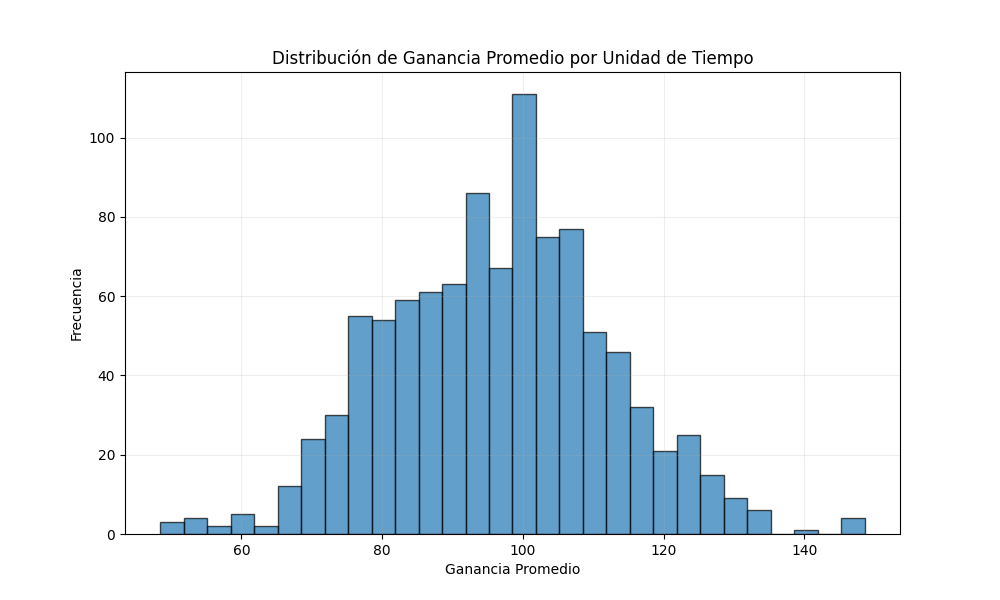
\includegraphics[width=0.8\textwidth]{images/Ganancia promedio por unidad de tiempo.png}
    \caption{Distribución de la ganancia promedio por unidad de tiempo}
\end{figure}

\subsection{Análisis de Sensibilidad (s, S)}

Los siguientes gráficos muestran el resultado luego de variar los parámetros
s y S para obtener resultados sobre cual sería la mejor combinación para el propietario en cuanto al 
aumento de las ganancias. De estos se deduce que la mejor combinación es: $s=30$ y $S=60$.

\begin{figure}[h]
    \centering
    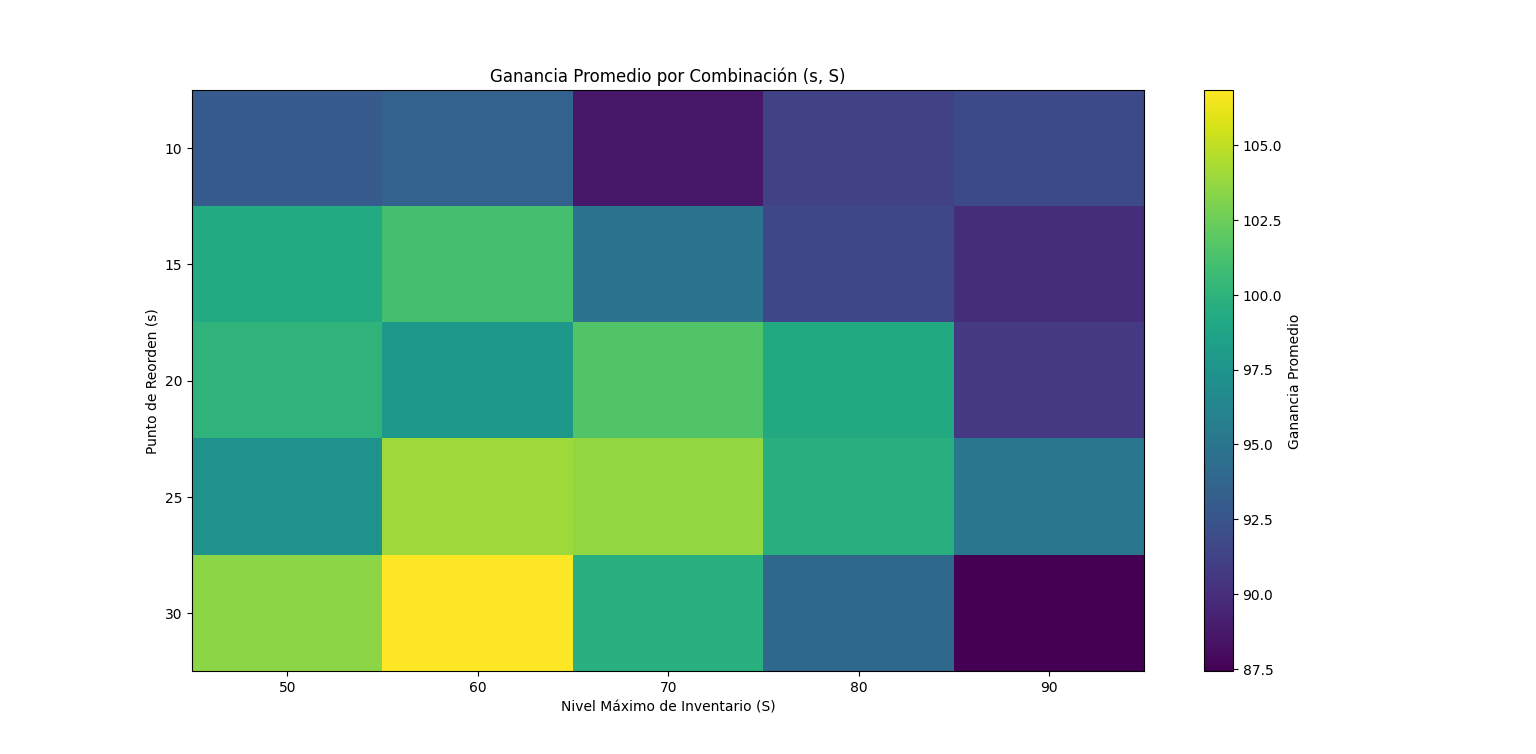
\includegraphics[width=0.8\textwidth]{images/Ganancia Promedio por Combinacion (s,S).png}
    \caption{Heatmap de ganancia promedio para diferentes combinaciones (s, S)}
\end{figure}

\begin{figure}[h]
    \centering
    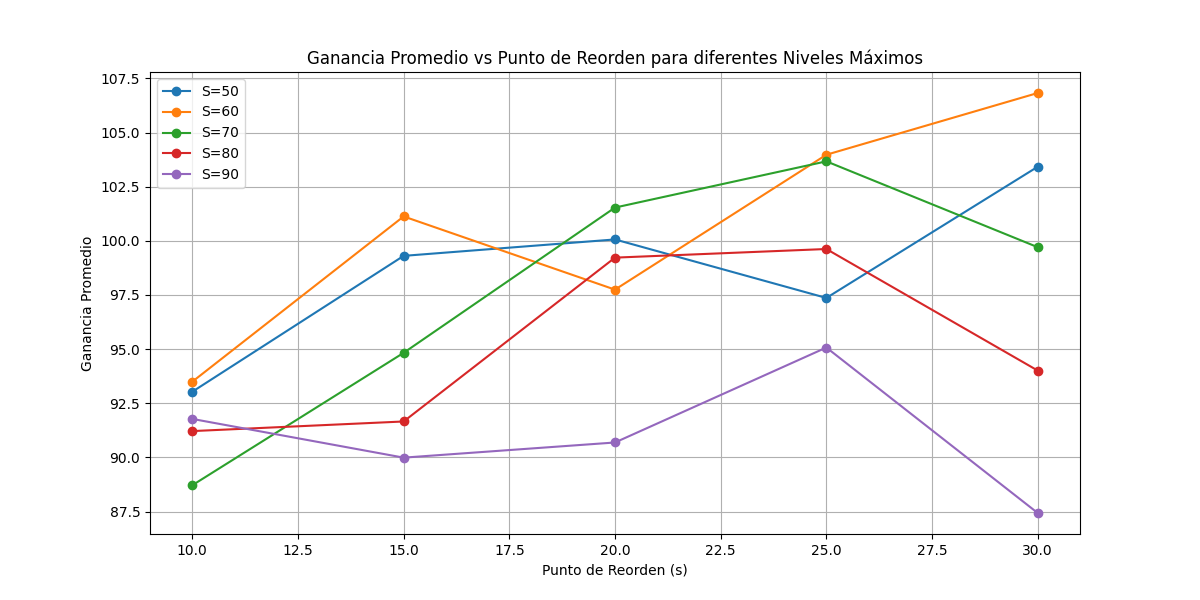
\includegraphics[width=0.8\textwidth]{images/Ganancia Promedio por Combinacion(s,S) por puntos.png}
    \caption{Heatmap de ganancia promedio para diferentes combinaciones (s, S)}
\end{figure}

\newpage
\subsection{Desglose de Costos e Ingresos}

\begin{tabular}{|c|c|c|}  % Columnas centradas (c) con bordes verticales (|)
    \hline                       % Línea horizontal
    \textbf{Campo}                          & \textbf{Valor} \\ \hline
    Ingresos Totales Promedio               & 4931.26         \\ \hline
    Costo de Pedidos Promedio               & 1703.04          \\ \hline
    Costo de Mantenimiento Promedio         & 912.59          \\ \hline
    Ganancia Promedio por Unidad de Tiempo  & 96.48          \\ \hline
    \end{tabular}

\begin{figure}[h]
    \centering
    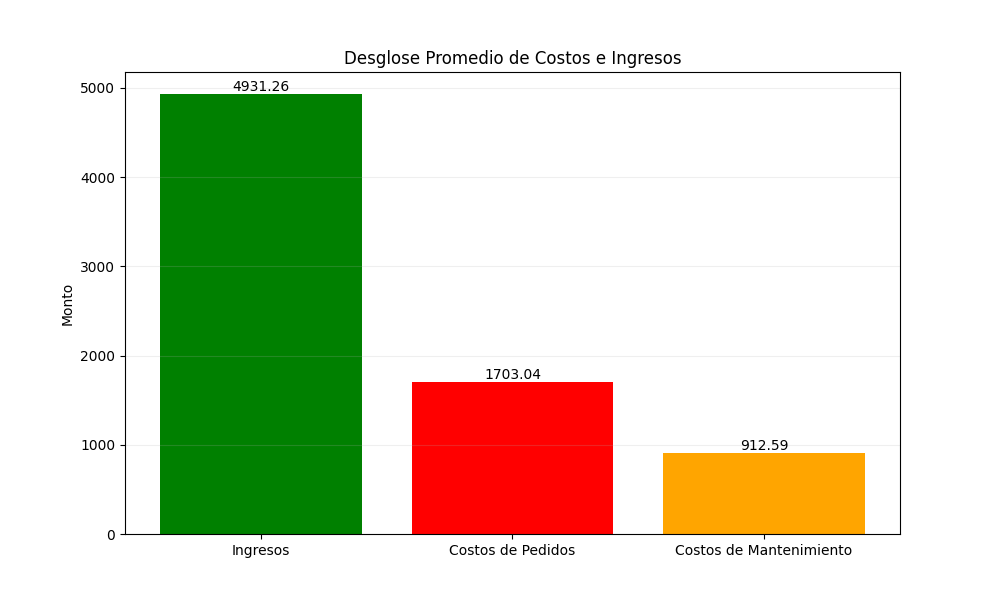
\includegraphics[width=0.6\textwidth]{images/Desglose Promedio de costos e Ingresos.png}
    \caption{Desglose promedio de costos e ingresos}
\end{figure}


\newpage
\section{Modelo Matemático}

\subsection{Formulación del Modelo}
El sistema puede modelarse como un proceso estocástico con:
\begin{align*}
\text{Beneficio} &= \text{Ingresos} - \text{Costos de Pedido} - \text{Costos de Mantenimiento} \\
\text{Ingresos} &= \sum_{i=1}^{N} \min(D_i, I(t_i)) \cdot p \\
\text{Costos de Pedido} &= \sum_{j=1}^{M} C(q_j) \\
\text{Costos de Mantenimiento} &= h \cdot \int_{0}^{T} I(t) dt
\end{align*}
donde:
\begin{itemize}
    \item $D_i$: Demanda del i-ésimo cliente
    \item $I(t)$: Nivel de inventario en tiempo $t$
    \item $p$: Precio de venta por unidad
    \item $q_j$: Cantidad del j-ésimo pedido
\end{itemize}

\subsection{Validación del Modelo}
La siguiente imagen muestra la comparación entre las distribución
de llegadas de los clientes con una distribución Poisson, de la cual se
puede observar que están bien aproximadas.
\begin{figure}[h]
    \centering
    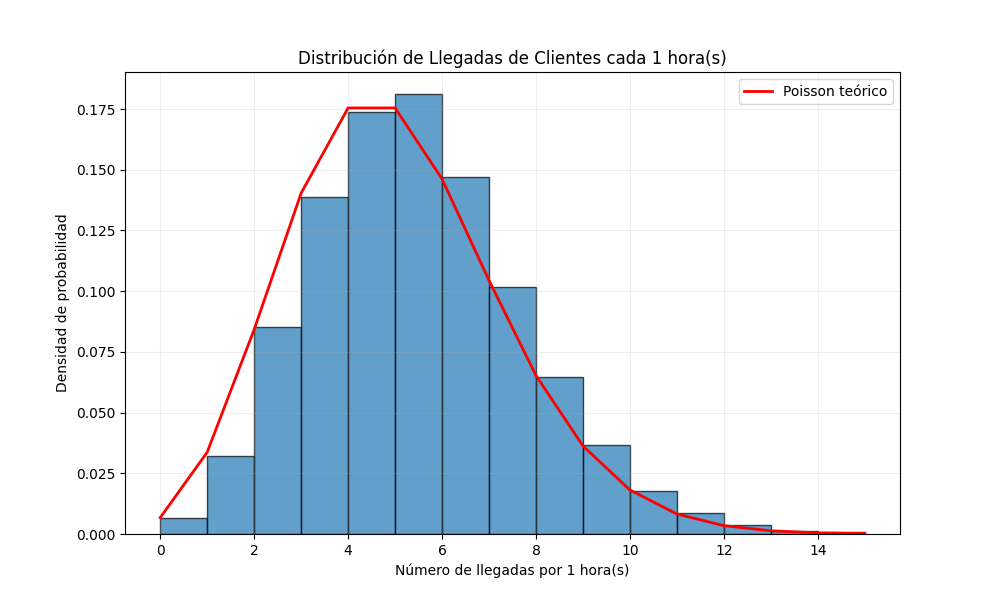
\includegraphics[width=0.8\textwidth]{images/Distribucion de Llegadas de Clientes en n horas.png}
    \caption{Distribución de llegadas de clientes vs distribución teórica Poisson}
    \label{fig:arrivals}
\end{figure}

\newpage
\section{Conclusiones}

\begin{itemize}
    \item La política óptima encontrada fue $s=30$, $S=60$ con ganancia promedio de 106.8 unidades por tiempo.
    \item La distribución empírica de llegadas coincide con el modelo teórico Poisson.
    \item El sistema es sensible a cambios en los parámetros (s, S).
\end{itemize}

\end{document}